% ============================================================================
% GALOSH — arXiv 原稿 v2 日本語版（再センタリング版、2026-07-02）
% galosh_paper.tex の対訳（確認・査読用。投稿は英語版）。
% pandoc で HTML 化: pandoc galosh_paper_ja.tex -o galosh_paper_ja.html
%   --standalone --embed-resources --mathml
% ============================================================================
\documentclass[10pt,twocolumn]{article}
\usepackage[margin=0.85in]{geometry}
\usepackage{booktabs}
\usepackage{graphicx}
\usepackage{amsmath,amssymb}
\usepackage[hidelinks]{hyperref}
\usepackage{xcolor}
\usepackage{caption}
\captionsetup{font=small}

\title{\textbf{GALOSH: 並列フレンドリな局所シュリンケージによる\\
Raw Bayer・sRGB 画像のブラインド・学習不要デノイジング}}
\author{Yoshiro Sato\thanks{本稿記載の手法を対象とする米国仮特許出願済み
（App.\ No.\ 64/058,343、2026 年 5 月 6 日）。}}
\date{}

\begin{document}
\maketitle

% ----------------------------------------------------------------- Abstract
\begin{abstract}
BM3D や non-local means のような学習不要の古典的デノイザは、その強さの多くを
\emph{探索}に負っている。内容依存のブロックマッチングは、メモリアクセスが不規則で
制御フローがデータ依存になるため並列化しにくく、固定レイテンシの実装を阻む。
学習ベースのデノイザは品質では最良だが、学習データを必要とし、学習ドメインの外
では劣化し（本稿でも実測される）、ピクセルあたり数万 MAC の計算量で事実上 GPU を
前提とする。本稿では \textbf{GALOSH}（Generalized Anscombe LOcal SHrinkage）を
提案する。これは探索を丸ごと取り除き、「マルチドメイン × 高速 × 高品質」を同時に
狙う学習不要デノイジングの再設計である：画像ごとの
ブラインド Poisson--Gaussian ノイズ推定、一般化 Anscombe 変換、輝度の 2 パス局所
Walsh--Hadamard シュリンケージ、輝度ガイドの色差局所回帰 --- 知覚的に異なる
2 つのノイズ成分（輝度の粒状感と色差の色むら）に対して意図的に異なる演算子を
充て、それぞれ独立の強度制御を持つ。全ステージが局所的・
データ非依存・規則的であり、どの画像のどのピクセルでも同一の計算グラフが走る。
一つのコアが 2 つのドメイン --- raw Bayer モザイクと sRGB/YUV 画像 --- を扱う。
実ノイズ 4 ベンチマーク（SIDD Medium と RawNIND の raw・sRGB）で、GALOSH は
blind・training-free 手法として一貫して最良であり、オラクルのノイズレベルを
与えた BM3D/NLM 系すら上回る。raw では学習済みネットワークに肉薄し、sRGB の
高 ISO ではドメイン内学習済みネットワークが依然上位であることも正直に報告する。
探索がないため高速である：フルベンチマークサイズにおいて同一 GPU 上で DL
ベースラインの $7\times$〜$650\times$ 高速（ドメイン依存。16\,MP raw フレーム
あたり 0.76\,s 対 5.6\,s、15.8\,MP sRGB フレームあたり 0.87\,s 対
13.5--565\,s）、かつ比較手法中で唯一、通常の CPU でも実用速度で動く。固定されたデータ非依存の構造は固定小数点・ストリーミング
ハードウェアへ自然に写像するよう設計されており、演算数解析と動作する INT16
固定小数点実現でこれを裏付ける。
\end{abstract}

% ----------------------------------------------------------------- Intro
\section{はじめに}
画像デノイジングには二つの系譜がある。\emph{古典的}な学習不要手法 ---
BM3D~\cite{bm3d} と non-local means~\cite{nlm} --- はデータ不要でセンサを
横断して一般化するが、既知のノイズレベルを前提とし、その品質を内容依存の
\emph{探索}で買っている。ブロックマッチングと近傍重み付けの不規則なメモリ
アクセスとデータ依存制御フローは、ベクトル化・GPU 占有率・固定レイテンシ予算の
いずれにも抵抗する。\emph{学習ベース}の手法（教師あり・自己教師ありの CNN や
Transformer）は学習したドメインでは優れた品質に達するが、学習ペアを必要とし、
ピクセルあたり数万 MAC を要し、学習分布の外では劣化する --- ときに壊滅的に
（\ref{sec:srgb}節）。

本稿の問いはこうである：探索を\emph{設計によって}取り除いたとき、古典系の品質は
どこまで残るか？ GALOSH は、全ステージが局所的・規則的・データ非依存のパイプライン
で答える。ノイズモデルは画像自体からブラインドに推定され、一般化 Anscombe 変換
（GAT）~\cite{foi} が単一のグローバル閾値を画面全体で有効にし、輝度は
Walsh--Hadamard 分解上の 2 パス局所シュリンケージ（BayesShrink~\cite{bayesshrink}
のパイロット + 経験的 Wiener パス）で、色差は輝度ガイドの局所線形回帰
~\cite{loess,kopf} でデノイズされる。この輝度/色差分離は意図的である：輝度
ノイズは粒状感として現れテクスチャと共存できるが、色差ノイズは決して許容され
ない色むらとして現れる。そのため 2 つの経路は攻撃性の異なる別々の演算子を使い、
独立した強度制御を公開する。どのステージも内容に対するマッチング・探索・
分岐を行わない：計算グラフが固定なので自明に並列化でき、コストはピクセルあたり
定数になる。

この再設計はドメイン汎用である。同じコアが 2 つの入力を処理する：
\textbf{GALOSH-RAW} は Bayer モザイク上で（各クワッドの $2{\times}2$
Walsh--Hadamard 変換が輝度/色差分解を与える）、\textbf{GALOSH-YUV/RGB} は
レンダリング済み sRGB 画像上で（線形光 BT.709 変換が同じ分解を与える）。
貢献は以下の通り：
\begin{itemize}\itemsep2pt
\item 全ステージが局所的・規則的・データ非依存な、ブラインド・学習不要・
\emph{探索不要}のデノイジングパイプライン。共有コアと 2 つのドメイン前段
（raw Bayer と sRGB/YUV）を持つ（\ref{sec:method}節）。
\item 実ノイズ 4 ベンチマークにわたり、GALOSH が両ドメインで最良の blind・
training-free 手法であるという証拠 --- オラクル $\sigma$ を与えた古典的
ベースラインに対しても --- と、学習済みネットワークが依然優位な箇所の正直な
報告（\ref{sec:results}節）。
\item 探索不要性の実用価値を示す速度検証：単一 GPU で DL ベースラインの
$7\times$〜$650\times$ 高速（ドメイン依存）、CPU でも実用的、さらに演算数解析と
動作する INT16 実現に
より固定小数点ストリーミング実装への適合性を示す
（\ref{sec:speed}、\ref{sec:map}節）。
\end{itemize}

% ----------------------------------------------------------------- Background
\section{背景}
GALOSH は、それぞれ個別には確立された 4 つの古典的アイデアを合成する。
\emph{分散安定化}：Foi ら~\cite{foi} は raw センサノイズが Poisson--Gaussian で
正確にモデル化でき、単一フレームからフィットできることを示した。一般化 Anscombe
変換はそれをほぼ単位分散の Gaussian に写し、Makitalo--Foi~\cite{makitalo} が
その不偏の厳密逆変換を与える。
\emph{変換領域シュリンケージ}：BayesShrink~\cite{bayesshrink} は観測係数統計から
準最適な閾値を定め、パイロット推定を使う 2 パス目の経験的 Wiener は標準的な
精緻化である（BM3D の 2 段構成~\cite{bm3d} と同様）。
\emph{局所重み付き回帰}：LOESS~\cite{loess} はカーネル重みの下で低次局所多項式を
フィットし、guided/joint-bilateral 系~\cite{kopf,guidedfilter} は一方のチャネルで
他方を操舵する。
GALOSH の主張は単一の構成要素ではなく、それらを探索不要・完全ブラインド・
2 ドメインのパイプラインへ合成したことにある --- BM3D のブロックマッチングを
サイクルスピンされた局所変換で置き換え、既知 $\sigma$ の仮定を、GAT が単一の
有効なグローバル閾値へ変換する画像ごとのブラインドフィットで置き換える。

% ----------------------------------------------------------------- Method
\section{手法}\label{sec:method}
共有コア（\ref{sec:core}節）と 2 つのドメイン前段（\ref{sec:raw}、
\ref{sec:yuv}節）から成る。全パラメータは推定ノイズモデルから導出されるか
固定定数であり、画像ごとのチューニングはない。

\subsection{GALOSH core}\label{sec:core}
\paragraph{ブラインドノイズ推定。}
Poisson--Gaussian モデル
$\operatorname{Var}[x]=\alpha\,\mathbb{E}[x]+\sigma^2$ を、重なり合うブロック上の
局所 Laplacian 分散対局所平均のロバスト回帰（Foi 型推定器~\cite{foi}）でノイズ
フレームのみからフィットし、オラクルもキャリブレーションデータもなしに画像ごとの
$(\alpha,\sigma^2)$ を得る。

\paragraph{分散安定化（GAT）。}
一般化 Anscombe 変換
$f(x)=\tfrac{2}{\alpha}\sqrt{\alpha x+\tfrac38\alpha^2+\sigma^2}$ が信号依存
ノイズをほぼ単位分散へ写し、単一のグローバル閾値がフレーム全体で有効になる。
高域残差のチャネル別中央絶対偏差（MAD）が残差スケールを与える。逆変換は厳密な
不偏逆~\cite{makitalo} を用いる。

\paragraph{輝度の 2 パス局所シュリンケージ（LOSH）。}
輝度は、重なり合う $8{\times}8$ Walsh--Hadamard ブロック上のサイクルスピン
（stride-1）局所シュリンケージでデノイズされる：パス 1 はロバスト
BayesShrink~\cite{bayesshrink} 閾値でパイロットを作り、パス 2 はパイロット係数
から計算した経験的 Wiener ゲインを適用する。重なりブロックは窓付き overlap-add
で再結合される。これは BM3D の shrink-then-Wiener 2 段構成から、協調（探索）3-D
スタックを密なサイクルスピン局所変換で置き換えたもの --- 内容依存性を全て取り除く
一手である。

\paragraph{輝度ガイドの色差回帰。}
各色差プレーンは、デノイズ済み輝度上の 1 次局所重み付き回帰（Y ガイド
LOESS~\cite{loess}；bilateral カーネル~\cite{kopf} を持つ guided
filter~\cite{guidedfilter} と等価）でデノイズされる：各局所窓内でカーネル重みが
空間距離と輝度類似度を組み合わせ、MAP 正則化された傾き/切片が色差を輝度に回帰
する。マルチスケール残差ピラミッドが同じ演算子を大粒度の色むらへ拡張する。1 次
回帰はエッジで外挿するため、再構成された全色差値は局所入力色差レンジへクランプ
される（「デノイザは入力にない色を発明してはならない」）。

\paragraph{意図的な輝度/色差の非対称。}
輝度/色差分離はデータ形式上の都合ではなく、本設計の知覚的な核心である。残留する
輝度ノイズはフィルム的な粒状感として現れテクスチャと共存できるため、輝度経路は
変換領域で控えめにシュリンクし、高周波構造を保存する。色差ノイズは視覚的に決して
許容されない色むらとして現れるため、色差経路ははるかに攻撃的に平滑化する ---
それが安全なのは、回帰がデノイズ済み輝度構造に係留され、局所入力色差レンジへ
クランプされているからである。2 つの経路は独立した強度制御（$s_L$、$s_C$）を
公開する。本稿の全ベンチマークは固定デフォルト（画像ごとのチューニングなし）を
使うが、この制御により、成分ごとに粒状感の保持と平滑さのトレードオフを別々に
選べる。この非対称性こそ、古典的ベースラインに対する知覚指標（LPIPS/DISTS）の
マージンが PSNR のマージンよりはるかに大きい主要因である（\ref{sec:results}節）。
古典的手法のカラー版も同じ非対称を暗黙に認めている --- CBM3D はブロック
マッチングを輝度チャネルのみで行い、OpenCV の Color-NLM は輝度/色差で別々の
強度を公開する --- が、どちらもその後は全成分に同一の探索ベース演算子を適用
する。GALOSH は非対称を構造にまで高め、成分ごとに異なる演算子を用いる。

\subsection{GALOSH-RAW}\label{sec:raw}
raw 前段は Bayer モザイク上で直接、単一フォワードパスで動く。ブラインドフィット
と GAT（コア）の後、CFA 対応の無彩色ダークリファレンス（局所無彩色フロアの IRLS
推定）を減算し、\emph{stride-1 サイクルスピン} $2{\times}2$ Walsh--Hadamard 変換が
各 Bayer クワッドを 1 つの輝度プレーン $L$（フル解像度）と 3 つの色差プレーン
$C_1,C_2,C_3$（半解像度 --- CFA は色差を輝度の半分のレートでサンプルするため、
帯域制限に忠実）へ変換する。$L$ はコアの 2 パス LOSH を受け、色差プレーンは
半解像度でコアのガイド回帰を受けたのち、輝度ガイドの joint-bilateral EWA jinc
アップサンプリングでフル解像度へ戻される（クロスチャネル事前分布により色差エッジ
が輝度エッジへスナップする。jinc の負サイドローブは局所 $2{\times}2$ 入力ハルへの
クランプでアンチリンギングされる）。逆 WHT、ダーク復元、厳密逆 GAT により、
任意のデモザイク後段に渡せるデノイズ済み Bayer フレームが得られる。

\subsection{GALOSH-YUV/RGB}\label{sec:yuv}
第二の前段はレンダリング済み sRGB 画像を受け付ける（主 API。線形 RGB 入口も
自明）。入力は逆 sRGB ガンマで線形化されフルレンジ BT.709 YCbCr へ変換される。
Y 上のノイズは同じブラインド Poisson--Gaussian 推定器でフィットされる
（レンダリング後のノイズもトーンカーブを通して信号依存のままであり、GAT が一次
近似でそれを吸収する）。Y は GAT + コアの 2 パス LOSH を、Cb/Cr はフル解像度で
コアの Y ガイド回帰を受ける（このドメインでは色差がサブサンプルされないため WHT
もアップサンプリングも不要）。raw パイプラインから反映された同じ局所色差レンジ
クランプを適用し、出力は $[0,1]$ へクランプされて順変換チェーンを通って返される。
独立した色差ノイズモデルはない：分散安定化空間で一定に保たれる回帰正則化係数が
その役割を果たす。

% ----------------------------------------------------------------- Setup
\section{実験設定}\label{sec:exp}
\paragraph{データセット。} raw ドメイン：\textbf{SIDD Medium}~\cite{sidd}
（フル解像度スマートフォン Bayer 80 枚）と \textbf{RawNIND}~\cite{rawnind}
（カメラ横断 $512^2$ 実ノイズ raw クロップ 1493 枚）。sRGB ドメイン：同じ 2 セット
の sRGB 版（SIDD のペア sRGB をフルフレーム $\sim$15.8\,MP で；RawNIND を sRGB へレンダリング、
全 1493 クロップ）。

\paragraph{プロトコル：すべてブラインド。} 全手法がブラインドで走る ---
クリーン/ノイズペアなし、画像ごとのノイズオラクルなし。古典的ベースラインは入力
から $\sigma$ を推定し、GALOSH は自前のブラインドフィットを使い、DL ベースライン
は公開されている実ノイズ学習済み重みを使う。忠実度（PSNR/SSIM）は各ネイティブ
ドメインで、知覚指標（LPIPS~\cite{lpips}、DISTS~\cite{dists}、NIQE~\cite{niqe}）
は sRGB 上で計算する（raw 結果は画像ごとのメタデータでレンダリング）。

\paragraph{ベースラインは設計上ドメインごとに適切なものを使う。} raw と sRGB の
デノイジングは異なるタスクであり、適切なベースラインも異なる。したがって 2 つの
ドメインは異なる手法セットを使う：raw Bayer では CFA 対応手法（BM3D-CFA、
NLM-CFA、その VST 前段アブレーション、raw 学習の Blind2Unblind~\cite{b2u}）、
sRGB ではカラー画像手法（CBM3D、Color-NLM、self-guided filter、sRGB 学習の
NAFNet~\cite{nafnet}、Restormer~\cite{restormer}、SCUNet~\cite{scunet}）。
なお、古典系はそれ自体がドメインを横断して適応する --- BM3D と NLM は
ドメイン適合形で両方の列に現れる（モザイク上では BM3D-CFA/NLM-CFA、カラー画像
上では CBM3D/Color-NLM）。この適応性は古典系の美徳であり、GALOSH はそれを
保持する --- 単一の共有コアと薄いドメイン前段によって --- 一方、学習済み
ネットワークは学習データのドメインとレンダリングに縛られる。

% ----------------------------------------------------------------- Results
\section{結果}\label{sec:results}

\subsection{raw ドメイン}\label{sec:rawres}
表~\ref{tab:sidd_medium} と~\ref{tab:rawnind} が raw ベンチマークを報告する。
blind・training-free 手法の中で GALOSH は両データセットの知覚指標で大差の最良
（LPIPS $0.203$/$0.240$ 対 BM3D/NLM 系の $0.27$--$0.55$、共有 VST 前段の有無に
よらず）であり、PSNR/SSIM でも競争力がある。\emph{学習済み}の Blind2Unblind
参照に対しては、RawNIND で知覚ギャップの大半を学習なしで詰める（LPIPS $0.240$
対 $0.222$）。VST アブレーション行が優位性の源泉を分離する：古典的ベースライン
に GALOSH 自身の分散安定化前段を与えても改善はわずかであり、ギャップの正体は
ノイズモデル単体ではなく探索不要の局所シュリンケージアーキテクチャである。
図~\ref{fig:qual_rawnind} と~\ref{fig:qual_sidd} に代表的なクロップを示す。

\subsection{sRGB ドメイン}\label{sec:srgb}
表~\ref{tab:sidd_srgb} と~\ref{tab:rawnind_srgb} が sRGB ベンチマークを、
図~\ref{fig:qual_srgb_sidd} と~\ref{fig:qual_srgb_rawnind} が対応するクロップを
示す。観察は 3 点。

\textbf{(i) GALOSH はブラインド古典的手法に決定的に勝つ。} SIDD sRGB での差は
大きい（フルフレームで 35.01\,dB 対 27--29；LPIPS 0.314 対 0.53--0.72）：空間相関を持つ信号依存
のレンダリングノイズは、ベースラインの $\sigma$ 推定器と白色ノイズ仮定の両方を
打ち破る。

\textbf{(ii) 優位性はアルゴリズムであり、ノイズ推定ではない。} RawNIND の最も
ノイジーなサブセット（ISO\,$\geq$\,6400、$n{=}30$）で、CBM3D と Color-NLM を
3 種類の $\sigma$ ソース --- 自前のブラインド推定、GALOSH の推定器、そして
グラウンドトゥルースから計算した\emph{オラクル} $\sigma$ --- で再実行した。
オラクルを与えても CBM3D は 21.33\,dB / LPIPS 0.450、Color-NLM は 21.26\,dB /
0.488 にとどまり、いずれも GALOSH の完全ブラインドの 22.13\,dB / 0.413 を
下回る。古典的手法に完璧なノイズレベルを手渡してもギャップは閉じない。

\textbf{(iii) 学習済み DL に対する正直な非対称。} SIDD sRGB では SIDD 学習
ネットワークが大きく先行する（NAFNet 41.94\,dB）--- 自らの学習セット上なので
当然である。クロスドメインの RawNIND では集計値は接近して見えるが
（表~\ref{tab:rawnind_srgb}）、集計はすでにクリーンな低 ISO シーンに支配されて
いる。ISO 帯別の内訳（表~\ref{tab:rawnind_srgb_iso}）が正直な見方である：高 ISO
では学習済みネットワークが GALOSH をやや上回り（+0.3--0.7\,dB）、GALOSH は
古典系を $\sim$2\,dB 上回り、blind・training-free グループで唯一ノイズの増加と
ともに利得を伸ばし続ける手法である。別件として、NAFNet-SIDD は暗部 37 シーンで
数値発散する（生出力 $\pm10^3$）。GALOSH を含む他の全ベースラインは同じ入力で
安定である --- 固定された学習不要計算のロバスト性の利点である。

\subsection{速度}\label{sec:speed}
全計時は単一マシン（RTX 4070\,Ti + 32 コア CPU）でのフルベンチマーク画像
あたりの値であり、表~\ref{tab:sidd_medium}--\ref{tab:rawnind} と
表~\ref{tab:sidd_srgb}--\ref{tab:rawnind_srgb} のプラットフォーム分離
CPU/GPU 列として示す。表~\ref{tab:speed} は 1080p 同一入力での統制参考値で
ある。探索不要性は直接に効く。GPU では GALOSH は全比較で最速である：16\,MP
raw フレームあたり 0.76\,s 対 学習済み Blind2Unblind の 5.6\,s（$7\times$）、
15.8\,MP sRGB フレームあたり 0.87\,s 対 NAFNet 13.5\,s・SCUNet 17.6\,s・
Restormer 565\,s（VRAM 律速のタイル attention）--- $15$--$650\times$。学習
ベースラインが実用的でない CPU では、GALOSH の raw ビルドはフルフレームで
BM3D-CFA と NLM-CFA の $2$--$3\times$ 高速であり（表~\ref{tab:sidd_medium}）、
32 スレッド sRGB ビルド（フルフレーム 2.5\,s）は Color-NLM（2.8\,s）より
高速でありながら遥かに高い品質を出す。GALOSH は比較中で唯一、高品質・GPU 高速・CPU 実用を同時に満たす手法で
ある。$512^2$ では GPU 起動オーバーヘッドが支配的になり、CPU ビルドが同等に
実用的である（表~\ref{tab:rawnind}）。

% ----------------------------------------------------------------- Mapping
\section{並列・固定小数点への写像}\label{sec:map}
探索を取り除いた性質は計算グラフも固定する：全ピクセルが内容に関係なく同じ演算を
実行する。ハードウェア実装を主張することなく、その帰結を定量化する。

\paragraph{演算数。} raw パイプライン全体の計測で、GALOSH のコストはピクセル
あたり約 $3.4$k 積和 + 約 $140$ LUT/特殊演算で、解像度非依存（1080p で $3391$
対 4K で $3370$）--- BM3D/NLM の $3.9$--$6.4\times$ 下、学習ベースラインの
$18$--$360\times$ 下であり、全域で局所的・データ非依存のアクセスパターンを持つ。

\paragraph{固定小数点実現。} シュリンケージコアは純 INT16 ストレージ / INT32
アキュムレートの固定小数点形式を持つ。INT32 ストレージでは GPU ストリーミング
実装は INT32 CPU 参照と end-to-end で bit-exact に一致する（SIDD・RawNIND の
フルフレームで検証済み）。ラインバッファを INT16 ストレージ形式（輝度 Q10.5、
クロマ Q6.9）に狭めても両者は near-lossless（フルフレームで $\approx$58--65\,dB
PSNR --- 残差はまさにこのストレージ量子化そのもの）であり、品質は ---
GPU INT16 出力で直接測定して --- FP32 参照と 0.1--0.7\,dB 以内で一致する
（表~\ref{tab:sidd_medium}、\ref{tab:rawnind}）。出荷パスのどこにも
64 bit 演算は不要である（広い中間値はペア 32 bit パターンを使う）。

\paragraph{フィージビリティであって製品ではない。} MAC アレイのスループット
モデルによれば、$0.5$--$1$\,TMAC/s の固定機能演算 --- 現在の ISP 水準では控えめ
--- が実時間 1080p--4K を維持でき、オンチップ状態は最大垂直カーネルのライン
バッファで抑えられる（1080p・INT16 で $\sim$200\,KB）。これらはアルゴリズムの
設計特性（「固定小数点ストリーミングハードウェアへ自然に写像するよう設計されて
いる」）として提示する。そのようなステージを実際に構築・検証することは今後の
課題である。

% ----------------------------------------------------------------- Discussion
\section{議論と限界}
GALOSH は学習済みネットワークをそのドメイン内で打ち負かすものではなく、sRGB の
高 ISO では学習済みネットワークが依然として品質面でやや優位である。我々の主張は
最先端の品質ではなく、その組み合わせ --- ブラインド・学習不要・マルチドメイン・
探索不要並列・高速 --- を、オラクル条件下の古典系すら上回る品質で同時に満たす
ことにある。raw SIDD の PSNR は学習済み Blind2Unblind をわずかに下回ったままで
ある。ブラインド推定器は強く相関したレンダリングノイズを過小推定する（すべての
高域推定器と同様）。これは sRGB の結果が吸収しているが、除去はしていない。
$\alpha$ 推定の軽量な学習コレクタは予備実験で有望であり、後続研究に委ねる。
動画（時間方向）拡張は自然である --- 計算はすでにフレームごと定数である --- が
本稿では未評価である。

% ----------------------------------------------------------------- Conclusion
\section{結論}
古典的デノイジングから探索を取り除き、分散安定化されたサイクルスピン局所
シュリンケージと輝度ガイドの局所回帰で置き換えても、古典系の品質は保たれ、
実際にはそれを拡張する（オラクルノイズレベルでも上回る）。同時に計算は局所的・
規則的・データ非依存になり、したがって並列かつ高速になる。一つの学習不要コアが
raw Bayer モザイクとレンダリング済み sRGB 画像の両方を扱い、GPU で学習ベース
ラインの $7\times$〜$650\times$（ドメイン依存）で走り、CPU でも実用的であり、
固定小数点ストリーミング
ハードウェアへ自然に写像するよう設計されている。

\begin{thebibliography}{19}\small
\bibitem{bm3d} K.~Dabov, A.~Foi, V.~Katkovnik, and K.~Egiazarian, ``Image
denoising by sparse 3-D transform-domain collaborative filtering,'' \emph{IEEE
TIP}, 2007.
\bibitem{nlm} A.~Buades, B.~Coll, and J.-M.~Morel, ``A non-local algorithm for
image denoising,'' \emph{CVPR}, 2005.
\bibitem{foi} A.~Foi, M.~Trimeche, V.~Katkovnik, and K.~Egiazarian,
``Practical Poissonian-Gaussian noise modeling and fitting for single-image
raw-data,'' \emph{IEEE TIP}, 2008.
\bibitem{makitalo} M.~Makitalo and A.~Foi, ``Optimal inversion of the
generalized Anscombe transformation for Poisson-Gaussian noise,'' \emph{IEEE
TIP}, 2013.
\bibitem{bayesshrink} S.~G.~Chang, B.~Yu, and M.~Vetterli, ``Adaptive wavelet
thresholding for image denoising and compression,'' \emph{IEEE TIP}, 2000.
\bibitem{loess} W.~S.~Cleveland, ``Robust locally weighted regression and
smoothing scatterplots,'' \emph{JASA}, 1979.
\bibitem{kopf} J.~Kopf, M.~F.~Cohen, D.~Lischinski, and M.~Uyttendaele,
``Joint bilateral upsampling,'' \emph{ACM SIGGRAPH}, 2007.
\bibitem{guidedfilter} K.~He, J.~Sun, and X.~Tang, ``Guided image filtering,''
\emph{ECCV}, 2010.
\bibitem{b2u} Z.~Wang et al., ``Blind2Unblind: Self-supervised image denoising
with visible blind spots,'' \emph{CVPR}, 2022.
\bibitem{nafnet} L.~Chen, X.~Chu, X.~Zhang, and J.~Sun, ``Simple baselines for
image restoration,'' \emph{ECCV}, 2022.
\bibitem{restormer} S.~W.~Zamir et al., ``Restormer: Efficient transformer for
high-resolution image restoration,'' \emph{CVPR}, 2022.
\bibitem{scunet} K.~Zhang et al., ``Practical blind image denoising via
Swin-Conv-UNet and data synthesis,'' \emph{Machine Intelligence Research},
2023.
\bibitem{sidd} A.~Abdelhamed, S.~Lin, and M.~S.~Brown, ``A high-quality
denoising dataset for smartphone cameras,'' \emph{CVPR}, 2018.
\bibitem{rawnind} B.~Brummer and C.~De~Vleeschouwer, ``Natural image noise
dataset,'' \emph{CVPRW}, 2019.
\bibitem{lpips} R.~Zhang, P.~Isola, A.~A.~Efros, E.~Shechtman, and O.~Wang,
``The unreasonable effectiveness of deep features as a perceptual metric,''
\emph{CVPR}, 2018.
\bibitem{dists} K.~Ding, K.~Ma, S.~Wang, and E.~P.~Simoncelli, ``Image quality
assessment: Unifying structure and texture similarity,'' \emph{IEEE TPAMI},
2020.
\bibitem{niqe} A.~Mittal, R.~Soundararajan, and A.~C.~Bovik, ``Making a
`completely blind' image quality analyzer,'' \emph{IEEE SPL}, 2013.
\end{thebibliography}

% ----------------------------------------------------------------- Tables
% ============================================================================
% GALOSH — ベンチマーク表（日本語キャプション版）
% 必要: \usepackage{booktabs}
% 凡例: 太字 = blind/training-free 手法中で最良、\underline = 同2位。
%       Blind2Unblind は学習済みネットワークで上限参照としてのみ掲載。
% ============================================================================

% ---------------------------------------------------------------- SIDD Medium
\begin{table}[t]
\centering
\caption{\textbf{SIDD Medium}（80 枚のフル解像度実ノイズ Bayer 画像）における
raw 領域ブラインド・デノイジング。全手法が \emph{blind}（クリーン/ノイズ対なし、
画像ごとのノイズオラクルなし）かつ \emph{training-free}（Blind2Unblind を除く）。
太字 / \underline{下線} = blind・training-free 手法中の最良 / 2位。
$\uparrow$: 高いほど良い、$\downarrow$: 低いほど良い。}
\label{tab:sidd_medium}
\setlength{\tabcolsep}{2pt}
\footnotesize
\resizebox{\columnwidth}{!}{%
\begin{tabular}{l ccccc rr}
\toprule
 & & & & & & \multicolumn{2}{c}{時間\,(s)}\\
\cmidrule(lr){7-8}
手法 & PSNR$\uparrow$ & SSIM$\uparrow$ & LPIPS$\downarrow$ & DISTS$\downarrow$ & NIQE$\downarrow$ & CPU & GPU\\
\midrule
\multicolumn{8}{l}{\textit{GALOSH（提案）--- blind・training-free}}\\
\quad GALOSH FP32          & \textbf{48.13} & \textbf{0.9883} & \textbf{0.2030} & \textbf{0.1690} & 8.62 & 12.6 & 0.76\\
\quad GALOSH INT16\,$^{\dagger}$ & \underline{47.42} & \underline{0.9881} & \underline{0.2030} & \underline{0.1694} & \underline{8.62} & 103.6$^{\dagger}$ & 2.7\\
% GALOSH 数値 = canonical GPU パイプライン（jinc アンチリンギング）、SIDD-Medium 全80枚:
% FP32 = o32 GPU、INT16 = i16 GPU（lf=5 cf=9。r32 CPU 参照に対し near-lossless
% ~58-65 dB end-to-end（フルフレーム）= INT16 ストレージ量子化そのもの。
% INT32 ストレージなら GPU は r32 と bit-exact、2026-07-04 検証済み）。
% galosh_fp32 + vst_galosh は 2026-07-02 に GPU exe で再検証（_metrics_revst_gpu.json、失敗0）。
% GPU 時間: fp32/vst = 同一セッションの専用非競合計測、int16 = i16 campaign 平均。
\addlinespace[2pt]
\multicolumn{8}{l}{\textit{アブレーション --- 共通 VST 前段（ネイティブ推定なし）}}\\
\quad VST\,+\,GALOSH core   & 44.35 & 0.9765 & 0.2132 & 0.1761 & \textbf{8.57} & 15.3 & 0.74\\
\quad VST\,+\,BM3D-CFA      & 45.96 & 0.9851 & 0.2932 & 0.2778 & 11.36 & 40.5 & ---\\
\quad VST\,+\,NLM-CFA       & 40.36 & 0.9679 & 0.4048 & 0.4194 & 12.98 & --- & 1.6\\
\addlinespace[2pt]
\multicolumn{8}{l}{\textit{古典的手法 --- blind、ネイティブ MAD}}\\
\quad BM3D-CFA             & 46.74 & 0.9862 & 0.2725 & 0.2613 & 10.55 & 40.4 & ---\\
\quad NLM-CFA              & 42.32 & 0.9729 & 0.3791 & 0.3901 & 12.05 & 27.1 & 1.2\\
\midrule
\multicolumn{8}{l}{\textit{学習済み DL（上限参照、blind ではない）}}\\
\quad Blind2Unblind        & 49.07 & 0.9924 & 0.1169 & 0.1281 & 9.43 & --- & 5.6\\
\bottomrule
\end{tabular}}

\vspace{2pt}
{\footnotesize 画像あたりのフルサイズ時間をプラットフォーム別の列に分離
（同じ列同士のみ比較可能）。CPU 列はすべてシングルスレッド実装。「---」= その
プラットフォームでは未計測（BM3D に GPU 移植はなく、Blind2Unblind は CUDA
必須）。NLM-CFA：GPU = CUDA 実装、CPU = 同一 patch/search パラメータの skimage
参照実装（フルフレーム 12 枚の平均；RawNIND の CPU 値は 100 シーン標本の中央値）。GALOSH は両列に値を持つ
--- クロスプラットフォームの基準点である。$^{\dagger}$INT16 の品質はストリーミング
INT16 GPU パイプラインで直接測定した値。CPU 時間は正確性優先の INT32 参照実装
（INT16 出力に対し near-lossless、速度未最適化）、GPU 時間はストリーミング
i16 実装（\ref{sec:map}節参照）。}
\end{table}

% ---------------------------------------------------------------- RawNIND
\begin{table}[t]
\centering
\caption{\textbf{RawNIND}（1493 枚のカメラ横断 $512{\times}512$ 実ノイズクロップ）に
おける raw 領域ブラインド・デノイジング。プロトコルと強調は
表~\ref{tab:sidd_medium} と同じ。}
\label{tab:rawnind}
\setlength{\tabcolsep}{2pt}
\footnotesize
\resizebox{\columnwidth}{!}{%
\begin{tabular}{l ccccc rr}
\toprule
 & & & & & & \multicolumn{2}{c}{時間\,(s)}\\
\cmidrule(lr){7-8}
手法 & PSNR$\uparrow$ & SSIM$\uparrow$ & LPIPS$\downarrow$ & DISTS$\downarrow$ & NIQE$\downarrow$ & CPU & GPU\\
\midrule
\multicolumn{8}{l}{\textit{GALOSH（提案）--- blind・training-free}}\\
\quad GALOSH FP32          & \underline{30.49} & \underline{0.7908} & \textbf{0.2395} & \textbf{0.2127} & \underline{8.64} & 0.54 & 0.45\\
\quad GALOSH INT16\,$^{\dagger}$ & 30.17 & 0.7860 & \underline{0.2453} & \underline{0.2161} & \textbf{8.63} & 2.32$^{\dagger}$ & 0.35\\
\addlinespace[2pt]
\multicolumn{8}{l}{\textit{アブレーション --- 共通 VST 前段（ネイティブ推定なし）}}\\
\quad VST\,+\,GALOSH core   & \textbf{30.63} & \textbf{0.8163} & 0.2481 & 0.2198 & 8.65 & 0.49 & 0.60\\
% vst_galosh は 2026-07-02 に GPU exe（外部 α/σ² 対応後）で再実行：現行 anti-ringing
% パイプライン、1493/1493、err 0（ベンチ JSON から機械照合。
% benchmark/scripts/verify_table_numbers.py 参照）。
% GPU 時間 fp32/vst = 専用非競合計測（_revst_gpu_time_rawnind.json、150 シーン標本）。
\quad VST\,+\,BM3D-CFA      & 30.07 & 0.7792 & 0.4320 & 0.3563 & 13.04 & 2.29 & ---\\
\quad VST\,+\,NLM-CFA       & 29.03 & 0.7649 & 0.5452 & 0.4636 & 14.57 & --- & 0.68\\
\addlinespace[2pt]
\multicolumn{8}{l}{\textit{古典的手法 --- blind、ネイティブ MAD}}\\
\quad BM3D-CFA             & 30.28 & 0.7848 & 0.4268 & 0.3461 & 12.15 & 2.30 & ---\\
\quad NLM-CFA              & 29.54 & 0.7735 & 0.5190 & 0.4364 & 13.80 & 0.58 & 0.76\\
\midrule
\multicolumn{8}{l}{\textit{学習済み DL（上限参照、blind ではない）}}\\
\quad Blind2Unblind        & 30.68 & 0.7932 & 0.2215 & 0.2018 & 8.93 & --- & ---\\
\bottomrule
\end{tabular}}

\vspace{2pt}
{\footnotesize プラットフォーム分離は表~\ref{tab:sidd_medium} と同じ。$512^2$
では GPU の起動/同期オーバーヘッドが GALOSH で支配的になるため、CPU ビルドが
ここでは競争的である。$^{\dagger}$表~\ref{tab:sidd_medium} 参照。Blind2Unblind
の計時は事前キャッシュ読み込みのため省略。}
\end{table}

% ------------------------------------------- Speed（統制参考）
\begin{table}[t]
\centering
\caption{\textbf{統制解像度の速度参考値}：1080p（1920$\times$1080 Bayer）、
CPU（1 コア）と GPU（NVIDIA RTX 4070\,Ti）。速度の\emph{主比較}は
表~\ref{tab:sidd_medium}--\ref{tab:rawnind} のフルサイズ画像あたり CPU/GPU 列で
ある。ウォーム実測。GALOSH GPU はカーネルパイプライン（context+build
$\sim$90\,ms は初回のみで償却）、他は end-to-end。}
\label{tab:speed}
\setlength{\tabcolsep}{8pt}
\resizebox{\columnwidth}{!}{%
\begin{tabular}{l rr}
\toprule
手法 & CPU (1 コア) & GPU\\
\midrule
\multicolumn{3}{l}{\textit{GALOSH（提案）--- blind・training-free}}\\
\quad GALOSH FP32 (o / o32)        & 1.38 s & \textbf{18.2 ms}\\
\midrule
\multicolumn{3}{l}{\textit{古典的手法（blind）}}\\
\quad BM3D-CFA                     & 6.33 s & ---\\
\quad NLM-CFA                      & 3.21 s & 0.42 s\\
\midrule
\multicolumn{3}{l}{\textit{学習済み DL}}\\
\quad Blind2Unblind                & ---$^{\dagger}$ & 0.74 s\\
\bottomrule
\end{tabular}}

\vspace{2pt}
{\footnotesize GALOSH FP32（GPU）は 4K で 46\,ms、5K で 72\,ms までスケールし
--- 同一 GPU 上で NLM-CFA の約 23$\times$、Blind2Unblind の約 40$\times$ ---
CPU でも古典的ベースラインの $2$--$5\times$ 高速である（1.38\,s 対
3.21/6.33\,s）：両プラットフォームで最速である。$^{\dagger}$Blind2Unblind の
参照実装は CUDA 必須で CPU では動作しない。INT16 固定小数点版
（\ref{sec:map}節）は CPU/GPU スループットではなく固定小数点ストリーミング
ハードウェアへの写像を狙うため、速度エントリには含めない。}
\end{table}

% ============================================================================
% GALOSH — sRGB（GALOSH-YUV/RGB）ベンチマーク表（日本語キャプション版）
% 出典: benchmark/scripts/bench_yuv_srgb.py 全 BLIND 実行 2026-06-29
% 凡例は RAW 表と同じ: 太字 = blind・training-free 手法中で最良、下線 = 同2位。
% DL 行は学習済み参照グループ。
% ============================================================================

% ---------------------------------------------------------------- SIDD sRGB
\begin{table}[t]
\centering
\caption{\textbf{SIDD Medium sRGB}（80 シーン、\textbf{フルフレーム}
$\sim$15.8\,MP）における sRGB 領域ブラインド・デノイジング。全手法がフル画像で
実行される（DL はオーバーラップ $1024^2$ タイル推論；LPIPS/DISTS は $1024^2$
タイル格子の平均）。全手法が \emph{blind}：古典的手法は入力から
$\sigma$ を推定（skimage \texttt{estimate\_sigma}）、GALOSH は自前のブラインド
ノイズモデル、DL は公開されている実ノイズ学習済み重み。太字 / \underline{下線} =
blind・training-free 手法中の最良 / 2位。学習済み DL は上限参照
（NAFNet と Restormer は SIDD \emph{で}学習されている）。}
\label{tab:sidd_srgb}
\setlength{\tabcolsep}{2pt}
\footnotesize
\resizebox{\columnwidth}{!}{%
\begin{tabular}{l ccccc rr}
\toprule
 & & & & & & \multicolumn{2}{c}{時間\,(s)}\\
\cmidrule(lr){7-8}
手法 & PSNR$\uparrow$ & SSIM$\uparrow$ & LPIPS$\downarrow$ & DISTS$\downarrow$ & NIQE$\downarrow$ & CPU & GPU\\
\midrule
ノイズ入力                 & 25.69 & 0.424 & 0.790 & 0.380 & 5.86 & --- & ---\\
\addlinespace[2pt]
\multicolumn{8}{l}{\textit{blind・training-free}}\\
\quad \textbf{GALOSH-YUV（提案）} & \textbf{35.01} & \textbf{0.837} & \textbf{0.314} & \textbf{0.243} & \underline{5.41} & 2.50 & 0.87\\
\quad CBM3D                & 27.09 & 0.492 & 0.721 & 0.349 & 5.52 & 118.6$^{1t}$ & ---\\
\quad Color-NLM            & \underline{28.92} & \underline{0.656} & \underline{0.534} & \underline{0.290} & \textbf{4.57} & 2.79 & ---\\
\quad Guided filter        & 27.43 & 0.523 & 0.687 & 0.349 & 5.79 & 0.71 & ---\\
\midrule
\multicolumn{8}{l}{\textit{学習済み DL（参照）}}\\
\quad NAFNet-SIDD          & 41.94 & 0.942 & 0.167 & 0.154 & 7.69 & --- & 13.5\\
\quad Restormer-SIDD       & 40.94 & 0.935 & 0.181 & 0.175 & 8.05 & --- & 565$^{v}$\\
\quad SCUNet-real          & 36.09 & 0.902 & 0.252 & 0.234 & 9.30 & --- & 17.6\\
\bottomrule
\end{tabular}}

\vspace{2pt}
{\footnotesize フル 15.8\,MP フレームの画像あたり時間をプラットフォーム別の列
に分離。「---」= そのプラットフォームの実装なし（古典的ベースラインに GPU 移植は
なく、DL は CPU では非実用的）。DL の時間は fresh プロセスの warm 実行値
（長寿命プロセスでは GPU メモリの経時劣化で膨張する）。$^{v}$Restormer のタイル
attention は本 12\,GB GPU ではフルフレームで VRAM 律速。両プラットフォームを
持つのは GALOSH のみ：GPU = カーネルパイプライン、CPU = 32 スレッドビルド。
CPU 行は $^{1t}$（参照 CBM3D パッケージは実質シングルスレッド）を除き全 32
コア使用。}
\end{table}

% ---------------------------------------------------------------- RawNIND sRGB
\begin{table}[t]
\centering
\caption{\textbf{RawNIND レンダリング sRGB}（カメラ横断 $512^2$ クロップ全
1493 枚）における sRGB 領域ブラインド・デノイジング。プロトコルと強調は
表~\ref{tab:sidd_srgb} と同じ。本セットは低 ISO シーンが支配的（1493 中 684 が
ISO\,2000 未満）で、集計値がノイズ入力側へ圧縮される --- ISO 帯別の内訳は
表~\ref{tab:rawnind_srgb_iso} を参照。}
\label{tab:rawnind_srgb}
\setlength{\tabcolsep}{2pt}
\footnotesize
\resizebox{\columnwidth}{!}{%
\begin{tabular}{l ccccc rr}
\toprule
 & & & & & & \multicolumn{2}{c}{時間\,(s)}\\
\cmidrule(lr){7-8}
手法 & PSNR$\uparrow$ & SSIM$\uparrow$ & LPIPS$\downarrow$ & DISTS$\downarrow$ & NIQE$\downarrow$ & CPU & GPU\\
\midrule
ノイズ入力                 & 22.13 & 0.662 & 0.479 & 0.253 & 8.58 & --- & ---\\
\addlinespace[2pt]
\multicolumn{8}{l}{\textit{blind・training-free}}\\
\quad \textbf{GALOSH-YUV（提案）} & \textbf{23.33} & \textbf{0.841} & \textbf{0.265} & \textbf{0.227} & \textbf{7.12} & 0.077 & 0.012\\
\quad CBM3D                & \underline{22.49} & 0.720 & 0.396 & \underline{0.228} & 6.33 & 2.60$^{1t}$ & ---\\
\quad Color-NLM            & 22.48 & \underline{0.761} & \underline{0.353} & 0.225 & \underline{7.82} & 0.19 & ---\\
\quad Guided filter        & 22.50 & 0.724 & 0.402 & 0.236 & 8.62 & 0.012 & ---\\
\midrule
\multicolumn{8}{l}{\textit{学習済み DL（参照）}}\\
\quad NAFNet-SIDD          & 22.58$^{\dagger}$ & 0.832 & 0.279 & 0.237 & 10.13 & --- & 0.13\\
\quad Restormer-SIDD       & 23.63 & 0.873 & 0.207 & 0.206 & 9.46 & --- & 0.35\\
\quad SCUNet-real          & 23.42 & 0.861 & 0.250 & 0.247 & 10.35 & --- & 0.14\\
\bottomrule
\end{tabular}}

\vspace{2pt}
{\footnotesize プラットフォーム分離と脚注は表~\ref{tab:sidd_srgb} と同じ
（時間は $512^2$）。$^{\dagger}$NAFNet-SIDD は本セットの暗部 37 シーンで数値
発散（クリップ前のネットワーク生出力が $\pm10^3$ に達する。該当シーンの
PSNR\,$<$\,5）。発散シーンを除外した平均
は 23.05。GALOSH を含む他の全手法は同じ入力で安定。値はそのまま報告。}
\end{table}

% ---------------------------------------------------------------- per-ISO
\begin{table}[t]
\centering
\caption{RawNIND sRGB の \textbf{ISO 帯別}平均 PSNR (dB)。低 ISO ではシーンが
ほぼクリーンでどの手法もほとんど改善できない。デノイズが効く高 ISO では、
GALOSH は古典的手法を明確に上回り、学習済み DL は GALOSH をやや上回る。
表~\ref{tab:rawnind_srgb} の集計値はこの両方の効果を隠すため、内訳を報告する。}
\label{tab:rawnind_srgb_iso}
\setlength{\tabcolsep}{5pt}
\resizebox{\columnwidth}{!}{%
\begin{tabular}{l cccc}
\toprule
 & ISO$<$400 & 400--2k & 2k--12.8k & $\geq$12.8k\\
手法 & (290) & (394) & (374) & (435)\\
\midrule
ノイズ入力       & 23.60 & 24.68 & 21.57 & 19.32\\
\addlinespace[2pt]
\textbf{GALOSH-YUV（提案）} & \textbf{23.66} & \textbf{25.20} & \textbf{22.58} & \textbf{22.06}\\
CBM3D            & \textbf{23.66} & 24.89 & 21.85 & 20.10\\
\midrule
NAFNet-SIDD      & 19.97$^{\dagger}$ & 24.44 & 22.67 & 22.56\\
Restormer-SIDD   & 23.68 & 25.36 & 22.77 & 22.78\\
SCUNet-real      & 23.52 & 25.26 & 22.62 & 22.36\\
\bottomrule
\end{tabular}}

\vspace{2pt}
{\footnotesize 太字 = blind・training-free 手法中の最良。$^{\dagger}$暗部発散
ケース（表~\ref{tab:rawnind_srgb}）は大部分がこの帯に含まれる（37 件中 29 件。
残り 8 件は 400--2k 帯で、当該セルもわずかに押し下げている）。}
\end{table}


% ----------------------------------------------------------------- Figures
\begin{figure*}[t]
\centering
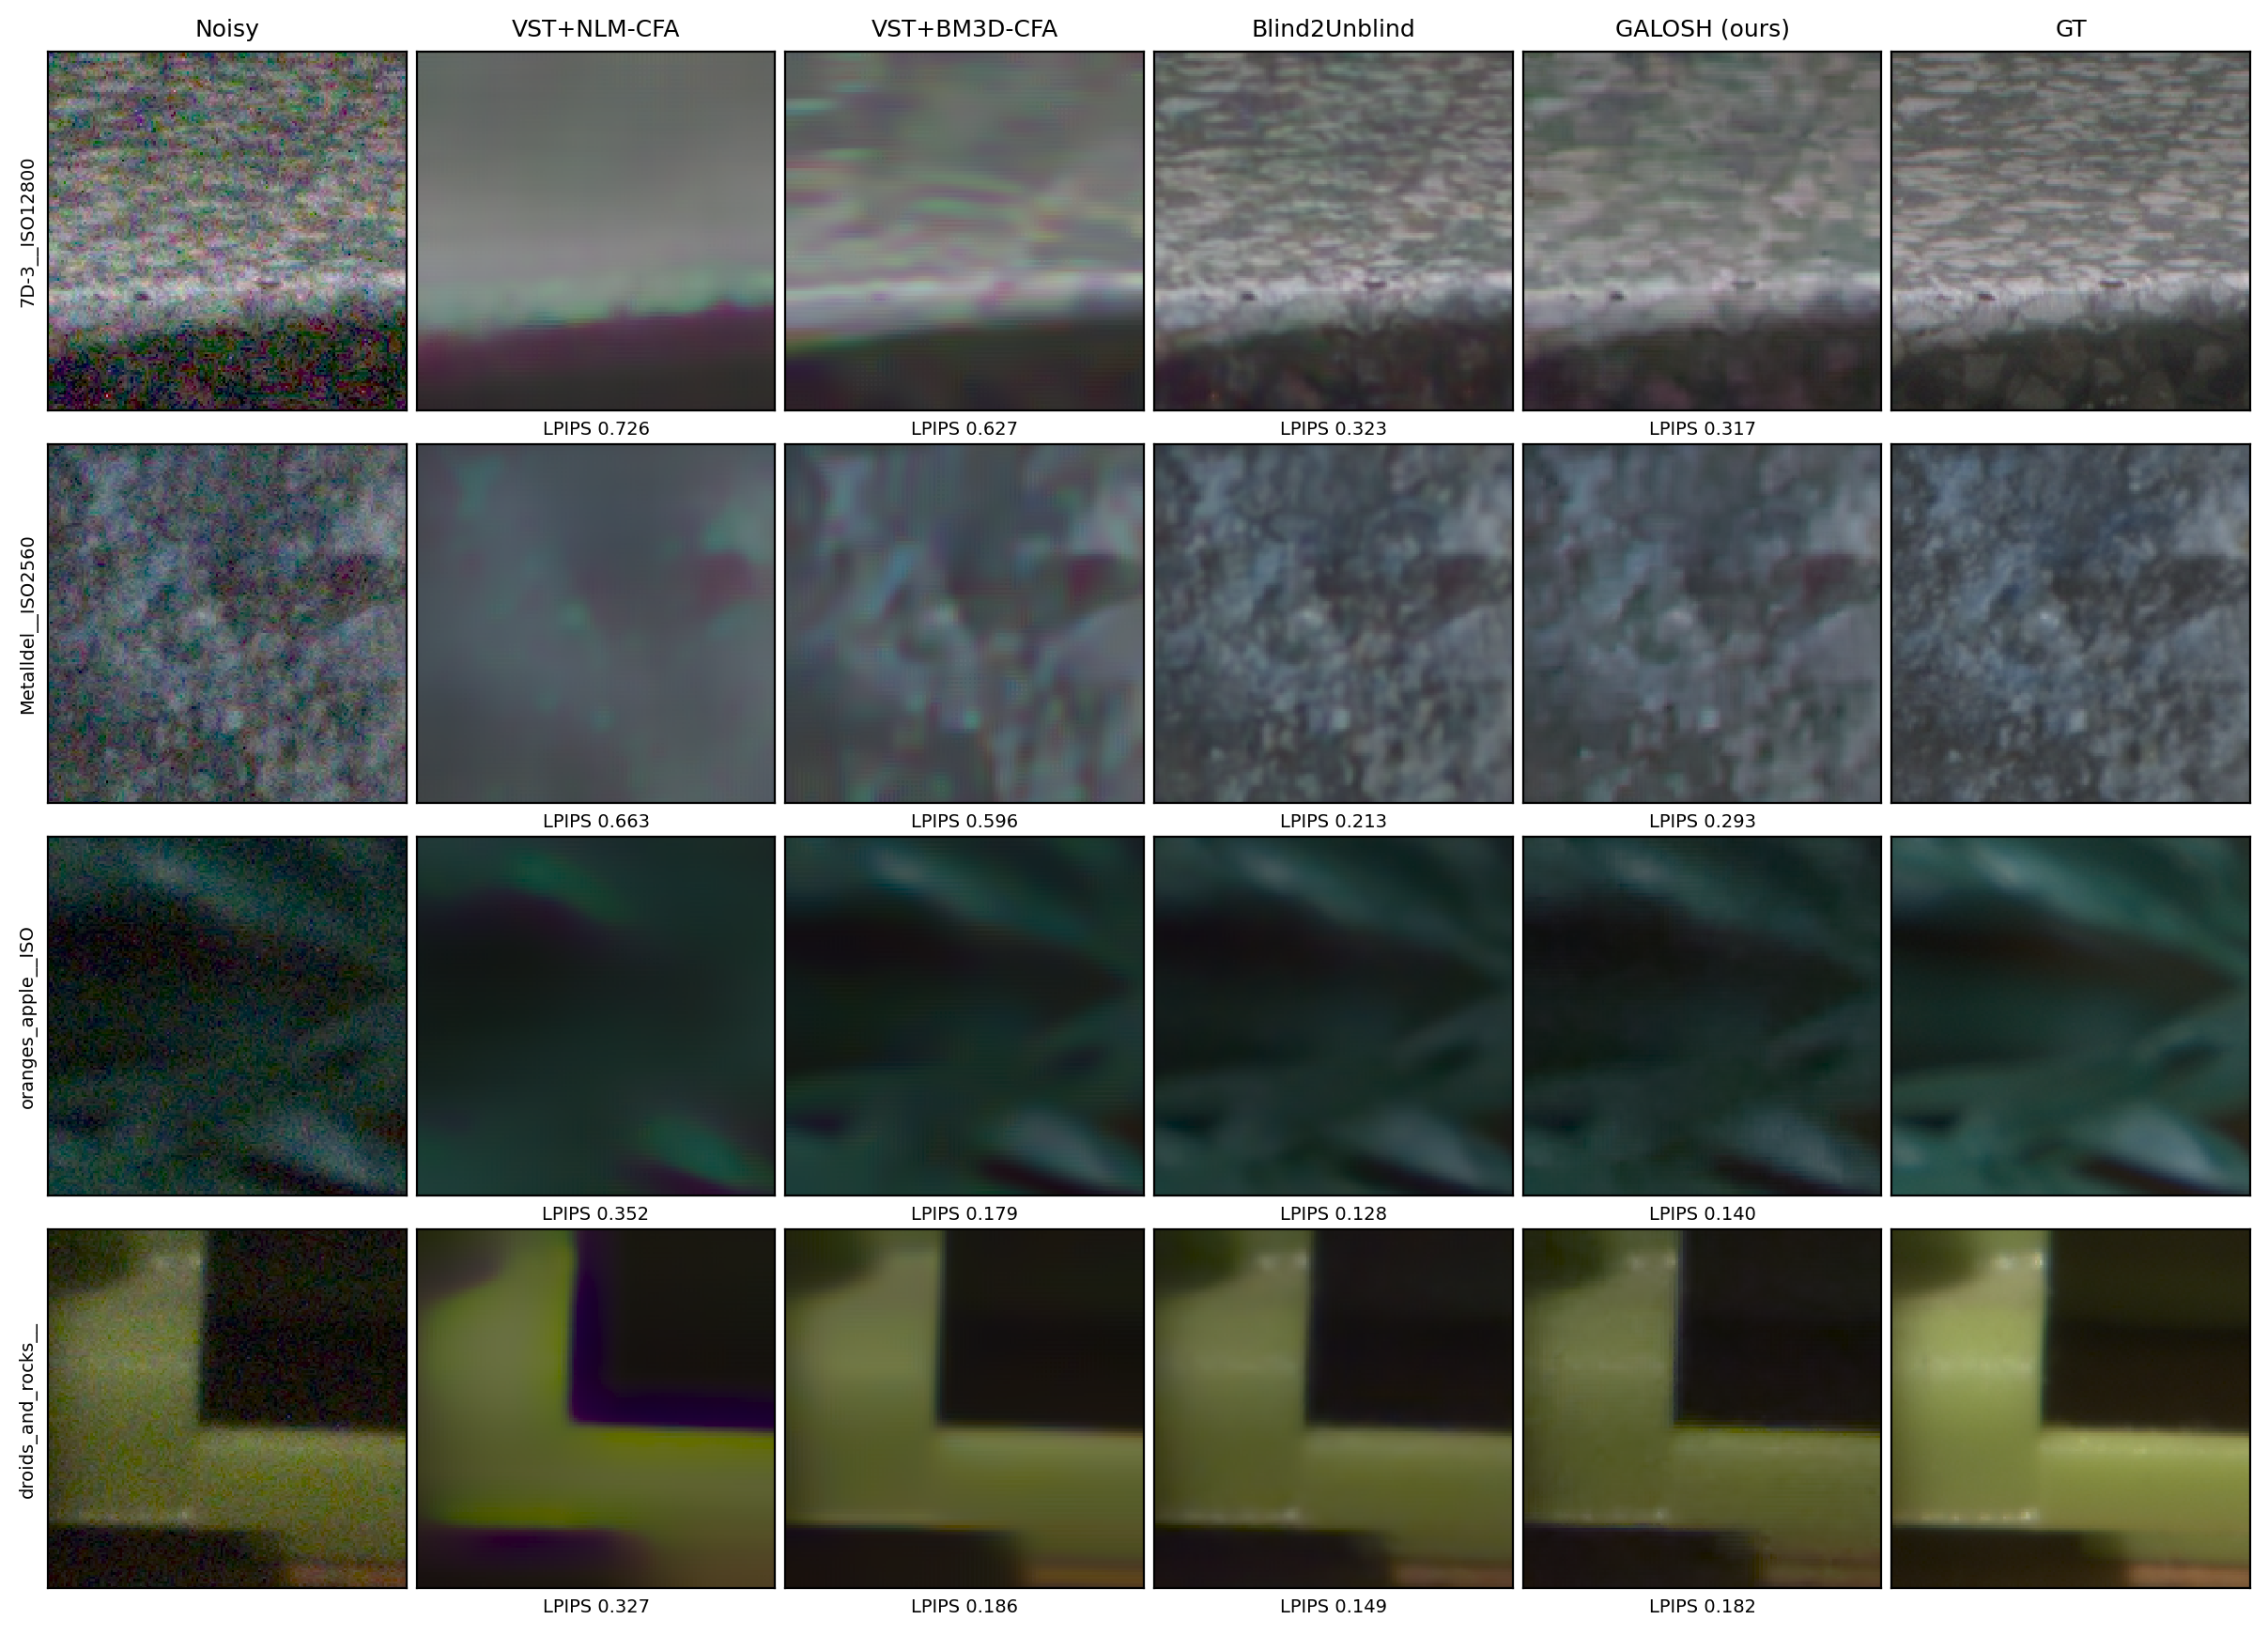
\includegraphics[width=\textwidth]{qualitative_rawnind.png}
\caption{raw ドメイン、RawNIND。列：Noisy / VST+NLM-CFA / VST+BM3D-CFA /
Blind2Unblind（学習済み）/ \textbf{GALOSH（提案、blind）} / GT。画像ごとの
LPIPS（$\downarrow$）付き。古典的ベースラインにはノイズ考慮の VST 前段を与えて
おり、GALOSH は完全ブラインドである。}
\label{fig:qual_rawnind}
\end{figure*}

\begin{figure*}[t]
\centering

\includegraphics[width=\textwidth]{qualitative_sidd_medium.png}
\caption{raw ドメイン、SIDD Medium（列は図~\ref{fig:qual_rawnind} と同じ）。}
\label{fig:qual_sidd}
\end{figure*}

\begin{figure*}[t]
\centering

\includegraphics[width=\textwidth]{qualitative_srgb_sidd.png}
\caption{sRGB ドメイン、SIDD Medium sRGB。列：Noisy / CBM3D / Color-NLM /
Guided / NAFNet-SIDD / SCUNet / Restormer-SIDD / \textbf{GALOSH（提案）} / GT。
画像ごとの LPIPS 付き。全手法ブラインド。古典的ベースラインは SIDD の相関した
レンダリングノイズに大きな残留ノイズを残し、GALOSH はそれらと SIDD 学習
ネットワークの間に位置する。}
\label{fig:qual_srgb_sidd}
\end{figure*}

\begin{figure*}[t]
\centering

\includegraphics[width=\textwidth]{qualitative_srgb_rawnind.png}
\caption{sRGB ドメイン、RawNIND（列は図~\ref{fig:qual_srgb_sidd} と同じ）。
行は ISO 12\,800--25\,600。中段：学習済みネットワークを含む全手法中で GALOSH の
LPIPS が最良となるケース。上段：学習済みネットワークが先行する暗所テキスト
シーン --- \ref{sec:srgb}節で論じた非対称である。}
\label{fig:qual_srgb_rawnind}
\end{figure*}

\end{document}
